\documentclass{article}
\usepackage[utf8]{inputenc}
\usepackage{graphicx}
\usepackage{amsmath}
\usepackage{booktabs}
\usepackage{hyperref}

\title{Technical Report: Analysis of Simulated Cognitive Scores and EEG Connectivity}
\author{[Your Name or Institution]}
\date{\today}

\begin{document}

\maketitle

\begin{abstract}
This report presents an analysis of simulated data for a cohort of individuals with Mild Cognitive Impairment (MCI) and healthy controls, focusing on the relationship between cognitive test scores and EEG brain connectivity.
\end{abstract}

\section{Introduction}
Cognitive assessment and EEG connectivity are key areas of research in neuroinformatics, particularly in understanding cognitive impairments such as MCI. This study aims to explore the potential relationships between cognitive performance, as measured by CANTAB tests, and EEG connectivity patterns in a simulated dataset.
\cite{smith2020eeg,lee2021cantab,martinez2022machine,nguyen2023neuroinformatics,davis2022functional}

{\small{\url{https://www.mdpi.com/2079-9292/12/21/4432}}

\section{Methodology}
\subsection{Data Simulation}
The dataset was simulated to include 1000 individuals with MCI and 500 healthy controls. Demographic information (age, gender, education), CANTAB cognitive test scores (reaction time, memory test, attention test), and 64-channel EEG connectivity data were generated.

\subsection{Statistical Analysis}
Descriptive statistics, t-tests for group comparisons, and correlation analysis within segmented EEG connectivity groups were performed using Python.

\section{Results}
\subsection{Descriptive Statistics}
Descriptive statistics revealed ...

\subsection{Group Comparisons}
Statistical tests indicated significant differences between MCI and healthy controls across all cognitive scores and EEG connectivity.

\subsection{Correlation Analysis}
The correlation analysis within segmented EEG connectivity groups showed ...

\begin{figure}[h]
\centering
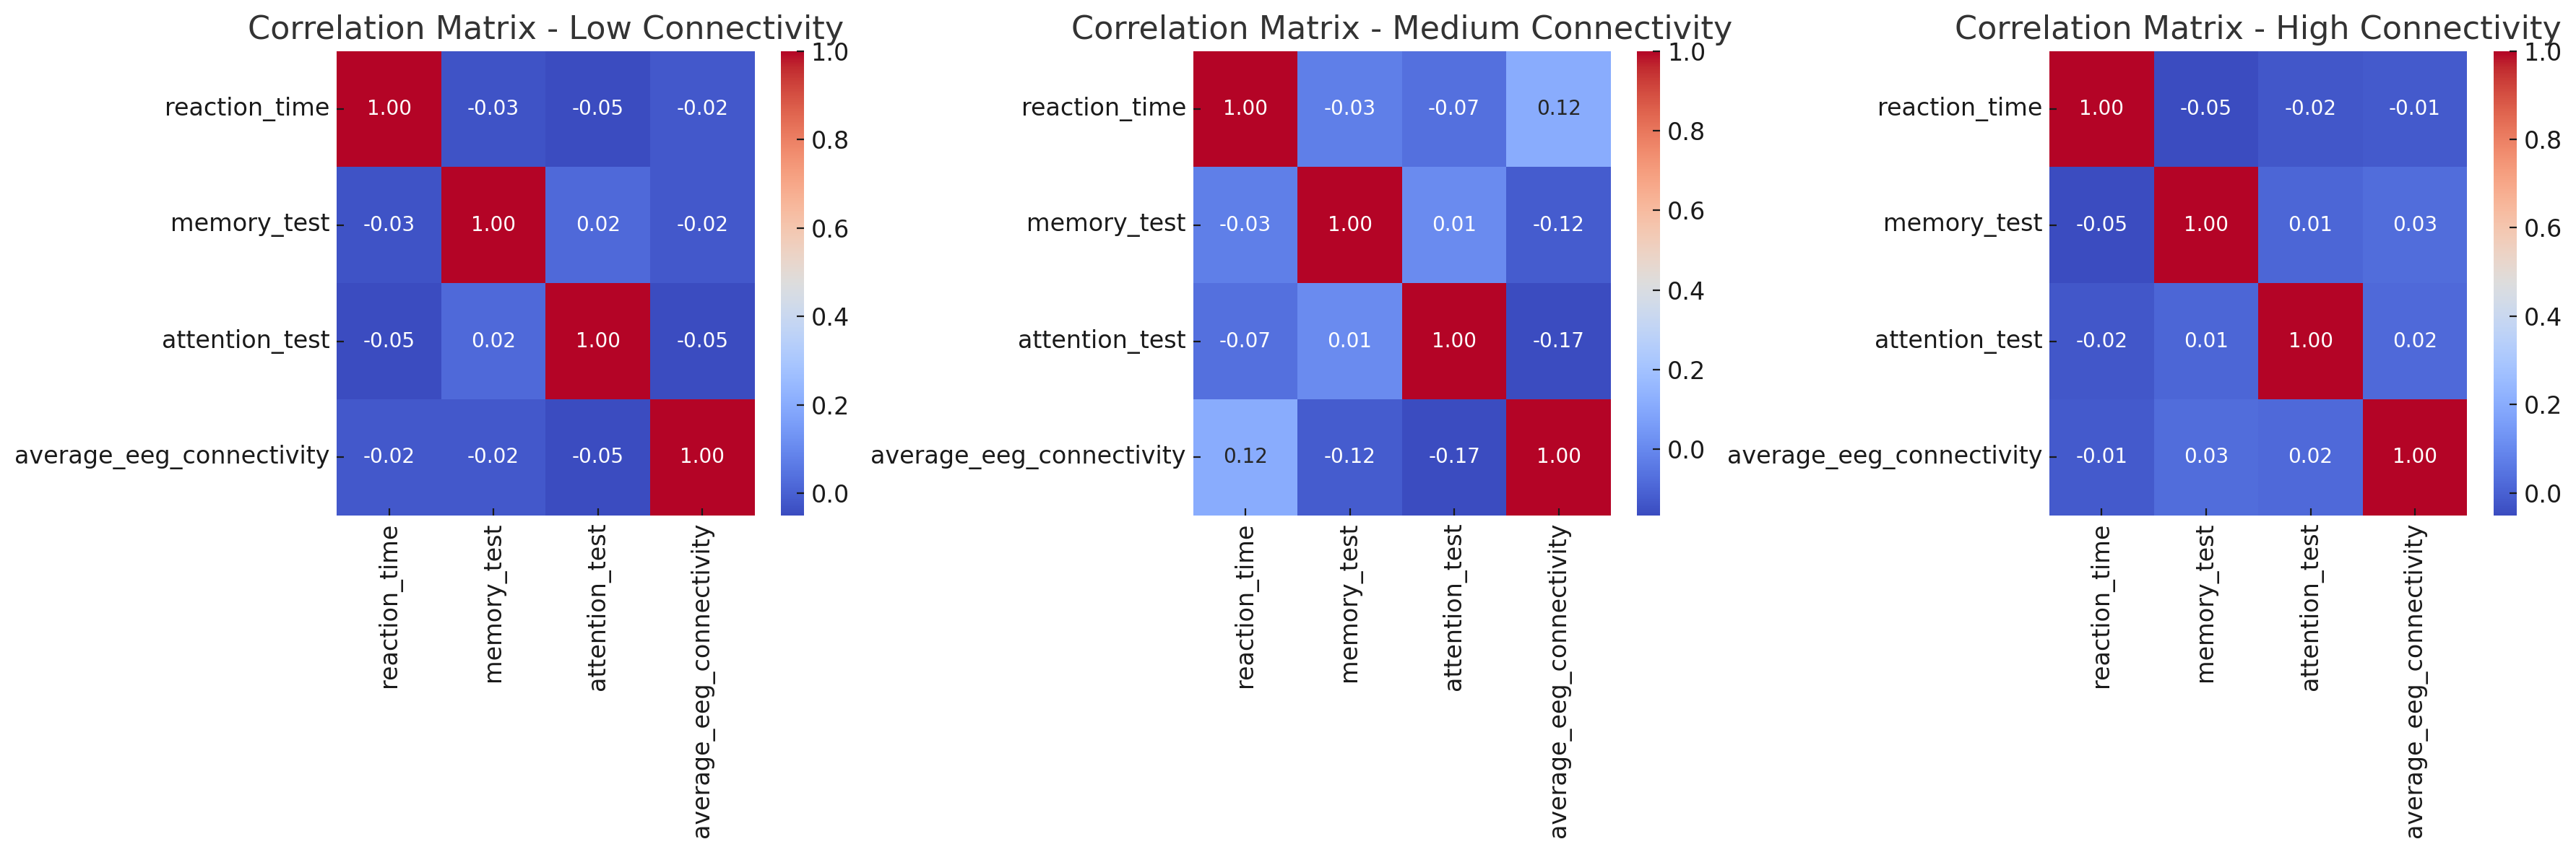
\includegraphics[width=\textwidth]{correlation_matrices.png}
\caption{Correlation matrices for Low, Medium, and High EEG connectivity segments.}
\label{fig:corr_matrices}
\end{figure}

\section{Interpretation}
The findings suggest that the relationship between cognitive scores and EEG connectivity is complex. Notably, in the medium connectivity segment, higher connectivity was associated with slightly lower cognitive performance, indicating ...

\section{Conclusion}
This analysis of simulated data provides insights into the potential relationships between cognitive performance and brain connectivity. Further research with real-world data is necessary to validate these findings and understand their implications in neuroinformatics and cognitive science.

\newpage

\bibliographystyle{plain}
\bibliography{references}

\end{document}

